%@descr: wzór sprawozdania, raportu lub pracy - nadaje się do przeróbek
%@author: Maciej Komosiński

\documentclass{article} 
\usepackage{polski} %moze wymagac dokonfigurowania latexa, ale jest lepszy niż standardowy babel'owy [polish] 
\usepackage[utf8]{inputenc} 
\usepackage[OT4]{fontenc}
\usepackage{graphicx,color} %include pdf's (and png's for raster graphics... avoid raster graphics!)
\usepackage{amsmath} %tylko dla \eqref
\usepackage{url}
\usepackage[pdftex,hyperfootnotes=false,pdfborder={0 0 0}]{hyperref} %za wszystkimi pakietami; pdfborder nie wszedzie tak samo zaimplementowane bo specyfikacja nieprecyzyjna; pod miktex'em po prostu nie widac wtedy ramek


% Zmiana rozmiarów strony tekstu
\addtolength{\voffset}{-1cm}
\addtolength{\hoffset}{-1cm}
\addtolength{\textwidth}{2cm}
\addtolength{\textheight}{2cm}

%bardziej zyciowe parametry sterujace rozmieszczeniem rysunkow
\renewcommand{\topfraction}{.85}
\renewcommand{\bottomfraction}{.7}
\renewcommand{\textfraction}{.15}
\renewcommand{\floatpagefraction}{.66}
\renewcommand{\dbltopfraction}{.66}
\renewcommand{\dblfloatpagefraction}{.66}
\setcounter{topnumber}{9}
\setcounter{bottomnumber}{9}
\setcounter{totalnumber}{20}
\setcounter{dbltopnumber}{9}

% własny bullet list z malymi odstepami
\newenvironment{tightlist}{
\begin{itemize}
  \setlength{\itemsep}{1pt}
  \setlength{\parskip}{0pt}
  \setlength{\parsep}{0pt}}
{\end{itemize}}

%obrazkow szukamy w nastepujacym katalogu:
\graphicspath{{pics/}}



%\title{Sprawozdanie z laboratorium:\\Metaheurystyki i Obliczenia Inspirowane Biologicznie}
%\author{}
%\date{}


\begin{document}

\thispagestyle{empty} %bez numeru strony

\begin{center}
{\large{Sprawozdanie z laboratorium:\\
Tutaj nazwa przedmiotu\\
(szablon)}}

\vspace{3ex}

Część I: Algorytmy optymalizacji lokalnej, problem QAP
%Część II: Algorytmy optymalizacji lokalnej i globalnej, problem QAP
%Część III: Eksperyment: ... (prezentację można zrobić w LaTeX - służy do tego klasa "beamer")

\vspace{3ex}
{\footnotesize\today}

\end{center}


\vspace{10ex}

Prowadzący: dr hab.~inż. Maciej Komosiński

\vspace{5ex}

Autorzy:
\begin{tabular}{lllr}
\textbf{Jan Kaczmarek} & inf80123 & ISWD & jasiu@serwer.domena.poczta.pl \\
\textbf{Ewa Kowalska} & inf89154 & PIESI & ewka@w.pl \\
\end{tabular}

\vspace{5ex}

Zajęcia poniedziałkowe, 11:00.

\vspace{35ex}

\noindent Oświadczam/y, że niniejsze sprawozdanie zostało przygotowane wyłącznie przez powyższych autora/ów,
a wszystkie elementy pochodzące z innych źródeł zostały odpowiednio zaznaczone i~są cytowane w bibliografii.  

\newpage


\section*{Udział autorów (jeśli $>1$)}
\begin{tightlist}
\item JK zaimplementował..., przeprowadził eksperyment..., opisał..., przygotował...
\item EK zaimplementowała..., przeprowadziła eksperyment..., opisała..., przygotowała...
\item Wszyscy autorzy przeczytali i zaakceptowali kompletne, ostateczne sprawozdanie.
\end{tightlist}

% Uwaga: wszyscy współautorzy muszą w całości przeczytać ostateczne sprawozdanie i je zaakceptować.
% (unikamy sytuacji gdzie np. X napisał program, Y przetestował i napisał sprawozdanie, X nie wie co Y napisał i jakie wnioski wyciągnał)



\section{Wstęp}

\begin{figure} %obrazek pojawia się przed pierwszym odwołaniem do niego -- to przydatna zasada
\begin{center}
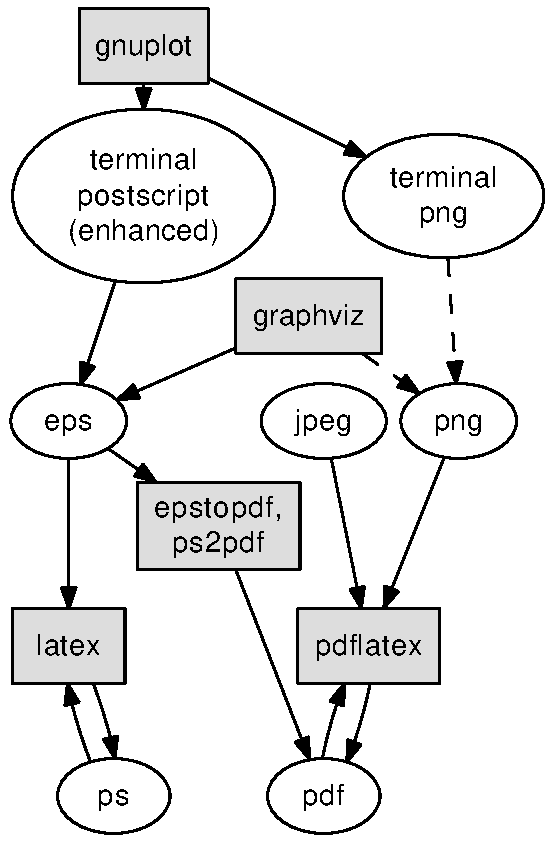
\includegraphics[width=0.4\textwidth]{rys_graf.pdf}
\end{center}
\caption{Przykładowy schemat z programu \emph{graphviz} -- narzędzia do automatycznego generowania schematów~\cite{graphviz}. Pamiętajmy, że wszędzie gdzie się da, używamy grafiki wektorowej -- unikamy wstawiania bitmap do dokumentu. W niektórych przypadkach użycie bitmap jest uzasadnione (w celu szybkiego podglądu na ekranie lub dla niezwykle skomplikowanych grafik, zawierających np.~setki tysięcy obiektów). Różnice w grafice rastrowej i wektorowej omawia prezentacja~\url{https://www.youtube.com/watch?v=_98SDNIpm24}.}
\label{fig:schemat}
\end{figure}


To jest przykładowy tekst w LaTeX. Przeczytaj go uważnie (treść, jego źródło oraz \%komentarze) i użyj tego źródła \texttt{*.tex} jako szablonu sprawozdania -- to źródło pokazuje jak

\begin{tightlist}
\item wstawić schemat stworzony graphviz'em (Rys.~\ref{fig:schemat}),
\item wstawić wykres stworzony gnuplot'em (Rys.~\ref{fig:3d}) oraz matplotlib'em (Rys.~\ref{fig:matplotlib}),
\item zacytować literaturę sformatowaną przez bibtex~\cite{MiOIBskrypt,Goldberg-2002},
\item odwoływać się do rysunków, cytowań i części sprawozdania (np.\ rozdział~\ref{sec:typografia}),
\item a także do równań: uwaga, najczęściej nie piszemy słowa ,,równanie'', piszemy tylko tak: W~\eqref{eq:tajemnicze-rownanie} pokazano zadziwiającą własność niektórych przekształceń matematycznych.
\end{tightlist}


\begin{equation}
\label{eq:tajemnicze-rownanie}
e^{i \pi} = -1 = \sqrt {-1} \sqrt {-1} = \sqrt {-1 \cdot -1} = \sqrt 1 = 1
\end{equation}


\section{Cechy dobrego sprawozdania}

Dobre sprawozdanie
\begin{tightlist}
\item pozwala odtworzyć samodzielnie czytelnikowi eksperyment (od danych po wyniki),
\item nie zawiera niedomówień,
\item przedstawia wnioski uporządkowane od ogólnych do szczegółowych,
\item cytuje literaturę w tekście,
\item nie zawiera zbyt obszernych listingów,
\item czytelnie prezentuje wyniki -- zwykle za pomocą wykresów,
\item wszelkie dane liczbowe pokazuje z właściwą liczbą miejsc znaczących,
\item jest zwięzłe i estetyczne.
\end{tightlist}

\subsection{Typografia}
\label{sec:typografia}

Pamiętajmy o różnicy pomiędzy łącznikiem\footnote{Przeczytaj w Wikipedii opis hasła ,,Dywiz''.} a myślnikiem -- a także o cytowaniu wszelkich materiałów źródłowych w odpowiednich miejscach~\cite{WikiDash}. Cytujmy konkretną stronę, a nie ogólny adres witryny. Cudzysłowy polskie piszemy metodą ,,przecinków i apostrofów''. Z kolei przy pojedynczych apostrofach rozróżniamy `otwierający i zamykający'.

Do sprawdzania pisowni bezpośrednio w pliku\ .tex służy między innymi program \emph{aspell}. Rozumie on różne sposoby kodowania polskich literek, a także ma wbudowane filtry do html'a i innych popularnych formatów. Dzięki tym filtrom pomija słowa kluczowe typowe dla danego formatu pliku, analizując tylko właściwy tekst. %backslash przed kropką i spacją podpowiada LaTeX'owi, żeby użył zwykłej spacji (a nie poszerzonej), ponieważ kropka za spacją nie jest końcem zdania (LaTeX domyślnie robi większe przerwy przed wszystkimi kropkami zakładając, że kropki oddzielają zdania).







\section{Wykresy}

\noindent Do przetwarzania tekstowych plików z wynikami oraz rysowania wykresów wyśmienicie nadaje się python wzbogacony o bibliotekę matplotlib. Zdecydowanie warto się ich nauczyć! Jeśli jednak chciał(a)byś wykorzystać program gnuplot (starsze narzędzie, nie polecam), to jego nowe wersje posiadają już niezły terminal `pdf', więc można zrezygnować z pośrednictwa formatu ps/eps. Jeśli nie wiesz jak zrobić jakiś rodzaj wykresu, sprawdź stronę z przykładami gnuplota~\cite{GnuplotDemos}.

Zanim przygotujesz wykres, obejrzyj koniecznie porady dotyczące ich tworzenia -- jak zrobić czytelny i profesjonalny wykres:~\url{https://www.youtube.com/watch?v=pfSgcsQ2Mtk}. %tylda to "nierozłączna spacja" -- skleja sąsiadujące wyrazy.



\begin{figure}
\begin{center}
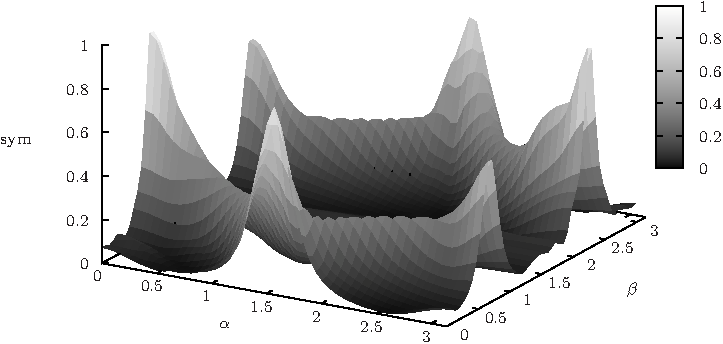
\includegraphics[width=0.9\textwidth]{rys_wykres3d.pdf}
\end{center}
\caption{Przykładowy wykres, ten akurat robiony przez program \texttt{gnuplot}.}
\label{fig:3d}
\end{figure}



\begin{figure}
\begin{center}
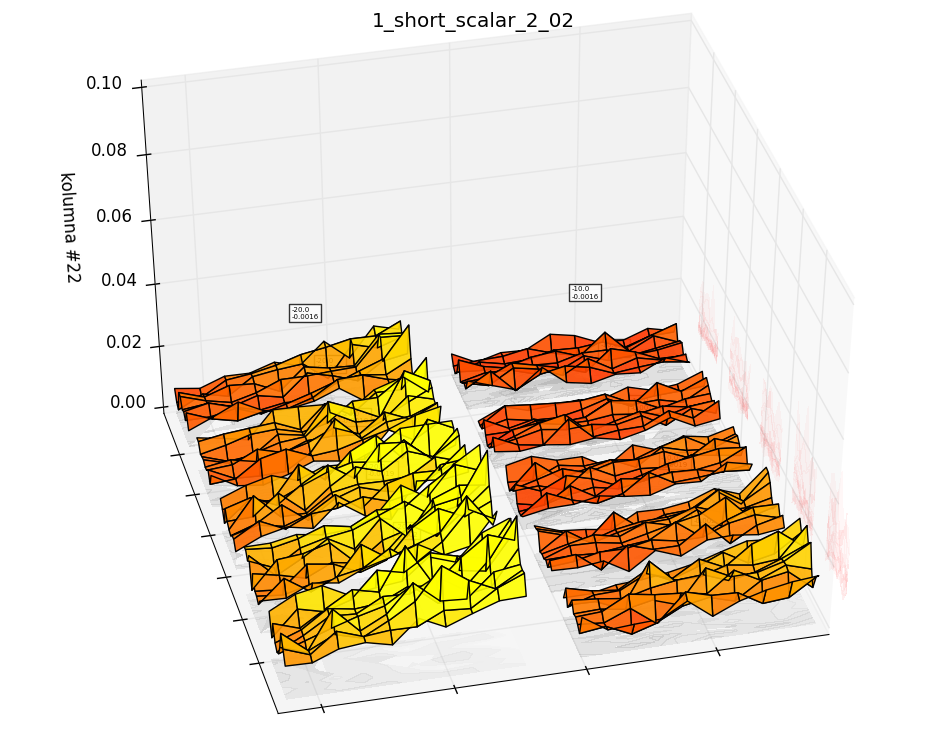
\includegraphics[width=0.48\textwidth]{rys_short_scalar_2_02.png}\hfill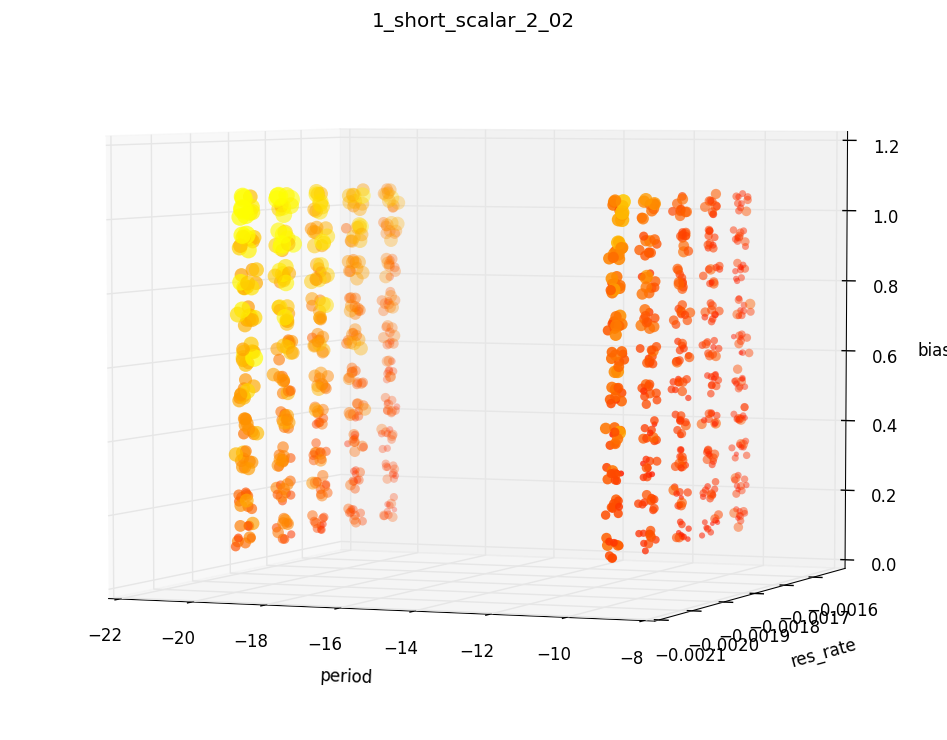
\includegraphics[width=0.48\textwidth]{rys_short_scalar_2_02-kulki.png}
\end{center}
\caption{Przykład wizualizacji w \texttt{python}+\texttt{matplotlib}; tutaj dane 5D pokazane na dwa sposoby w 3D. Co jest nie tak z tym rysunkiem? wstawione są bitmapy (nieprawidłowo, powinna być postać wektorowa), a wykresy są tu za małe (nieczytelne).}
\label{fig:matplotlib}
\end{figure}

\clearpage %pozwól LaTeX'owi umieścić zaległe rysunki od razu tutaj -- to polecenie "uwalnia" nagromadzone zaległości, co przydaje się jeśli umieściliśmy duużo obrazków, dużo więcej niż tekstu -- dzięki temu nie wylądują na końcu dokumentu



\section{Zakończenie}

A teraz coś na deser. Skoro przeczytałeś całe to źródło tekstu, rozpraw się z jednym niepozornym zdaniem: \url{http://www.mooncoder.com/latex-challenge.html} %i juz nigdy nie zapomnij, czym się różnią łączniki od myślników!


%%%%%%%%%%%%%%%% literatura %%%%%%%%%%%%%%%%

\bibliography{sprawozd}
\bibliographystyle{plainurl}


\end{document}
